%%%%%%%%%%%%%%%%%%%%%%% file typeinst.tex %%%%%%%%%%%%%%%%%%%%%%%%%
%
% This is the LaTeX source for the instructions to authors using
% the LaTeX document class 'llncs.cls' for contributions to 
% the Lecture Notes in Computer Sciences series.
% http://www.springer.com/lncs       Springer Heidelberg 2006/05/04
%
% It may be used as a template for your own input - copy it 
% to a new file with a new name and use it as the basis
% for your article. 
%
%%%%%%%%%%%%%%%%%%%%%%%%%%%%%%%%%%%%%%%%%%%%%%%%%%%%%%%%%%%%%%%%%%%


\documentclass[runningheads]{llncs}

\usepackage{amssymb}
\setcounter{tocdepth}{3}
\usepackage{graphicx}
\graphicspath{{../figures/}}

\usepackage{algorithm}
\usepackage{algorithmic}
\usepackage{tabularx}
\usepackage{multirow}
\usepackage{rotating}
\usepackage{comment}


\usepackage[latin1]{inputenc}
\usepackage{url}
\usepackage{epsf}
\urldef{\mailsa}\path|kartik@ee.iitb.ac.in|
\urldef{\mailsb}\path|gabriel.caffarena@ceu.es|
\urldef{\mailsc}\path|alberto.gilf@gmail.com|
\urldef{\mailsd}\path|david.gonzalez.marquez@usc.es|
\urldef{\mailse}\path|abraham.otero@gmail.com|
\urldef{\mailsf}\path|madhav@ee.iitb.ac.in|
\newcommand{\keywords}[1]{\par\addvspace\baselineskip
\noindent\keywordname\enspace\ignorespaces#1}


\def\NoNumber#1{{\def\alglinenumber##1{}\State #1}\addtocounter{ALG@line}{-1}}

\begin{document}

\mainmatter  % start of an individual contribution

% first the title is needed
\title{Low-latency Hermite Polynomial Characterization of Heartbeats using a Field-Programmable Gate Array}

% a short form should be given in case it is too long for the running head 
\titlerunning{Low-latency Hermite Polynomial Characterization using an FPGA}


% the name(s) of the author(s) follow(s) next
%
% NB: Chinese authors should write their first names(s) in front of
% their surnames. This ensures that the names appear correctly in
% the running heads and the author index.
%
\author{Kartik Lakhotia\inst{1} \and
 Gabriel Caffarena\inst{2} \and 
 Alberto Gil\inst{3} \and
 David G. Marquez \inst{3} \and 
 Abraham Otero\inst{2} \and
 Madhav P. Desai \inst{1}}

% if the list of authors exceeds the space for a headline,
% an abbreviated author list is needed
\authorrunning{Kartik Lakhotia et al.}
% (feature abused for this document to repeat the title also on left hand pages)



% the affiliations are given next
\institute{Indian Institute of Technology (Bombay), \\
Powai, Mumbai 400076, \\
India\\
\and 
University CEU-San Pablo,\\
Urb. Monteprincipe, 28668, Madrid, Spain\\
%\mailsa\\
\mailsb\\
%\mailsd\\
\url{http://biolab.uspceu.com}\\
%\mailsc\\
\and
Centro Singular de Investigacion en Tecnoloxías da Informacion (CITIUS),\\
University of Santiago de Compostela, 15782 Santiago de Compostela, Spain
}

%
% NB: a more complex sample for affiliations and the mapping to the
% corresponding authors can be found in the file "llncs.dem" 
% (search for the string "\mainmatter" where a contribution starts).
% "llncs.dem" accompanies the document class "llncs.cls".
%
\toctitle{Lecture Notes in Computer Science}
\tocauthor{Authors' Instructions}
\maketitle


\begin{abstract}
The characterization of ECG heartbeats is a computationally intensive problem, and
both off-line and on-line (real-time) solutions to this problem are of great interest.
In this paper, we consider the use of a field-programmable gate-array (FPGA) to solve
a critical component of this problem. We describe an implementation of
a best-fit Hermite approximation of a heartbeat using six Hermite polynomials.  
The implementation is generated using an algorithm-to-hardware compiler tool-chain
and the resulting hardware is characterized using an off-the-shelf FPGA card.
The single beat best-fit computation latency is under $0.5ms$ with a power dissipation of under 10 watts. 

\keywords{Hermite approximation, ECG, QRS, Arrhythmia,  FPGA, Parallelization}
\end{abstract}


\section{Introduction}

Automatic ECG analysis and characterization can help in 
identifying anomalies in a long-term ECG recording. 
In particular, the characterization of the QRS complex by means of Hermite functions 
seems to be a reliable mechanism  for automatic classification of heartbeats \cite{j:lagerholm00}. 
The main advantages seem to be the low sensitivity to noise and artifacts, and the
compactness of the representation (e.g. a 144-sample QRS can be characterized with 7 parameters \cite{c:marquez13}). 
These advantages have made the Hermite representation a very common tool for characterizing the 
morphology of the beats \cite{j:lagerholm00,c:marquez13,c:braccini97,j:linh03a,j:linh03b}. 

ECG analysis using Hermite functions has a
substantial amount of parallelism.  Solutions to the problem have been investigated
using processors (and multi-cores) and graphics processing units (GPU's). 
In this paper, we consider the alternative route of using an FPGA to implement
the computations.  In particular, our work is motivated by the potential
of an FPGA (or eventually, a dedicated application-specific circuit) for low-latency
energy efficient heart-beat analysis.  

In generating the hardware for heart-beat analysis, we make extensive use of
algorithm-to-hardware techniques.  By this we mean that the hardware is
generated from an algorithmic specification that is written in a
high-level programming language ({\bf C} in this case), which is then
transformed to a circuit implementation using a set of compiler tools \cite{c:ahir_thesis2009,c:ahir_dsd2010,c:ahir_usenix2012}.
The resulting hardware is then mapped to an FPGA card (the ML605 card from Xilinx,
which uses a Virtex-6 FPGA).  The circuit is then exercised through the PCI-express 
interface and used to classify beats.  The round-trip latency of a single
beat classification was found to be under $0.5ms$.

%\begin{itemize}
%\item The assessment of the capabilities of GPUs for the off-line characterization of heartbeats using Hermite functions approximations
%\item The assessment of the capabilities of GPUs for the on-line characterization of heartbeats using Hermite functions approximations
%\end{itemize}

\section{QRS approximation by means of Hermite polynomials}\label{s:arr}

The aim of using the Hermite approximation to estimate heartbeats is to 
reduce the number of dimensions required to carry out the ECG classification, 
without sacrificing accuracy. 
The benchmarks used in this work come from the MIT-BIH arrhythmia database \cite{j:moody01} which is made up of 
48 ECG recordings whose beats  have been manually annotated by two cardiologists. Each file from the database 
contains 2 ECG channels, sampled at a frequency of 360 Hz and with a duration of approximately 2000 beats. 
In particular, here we are addressing the characterization of the morphology of the QRS complexes since this 
morphology, together with the distance between each pair of consecutive heartbeats, permits the identification of the majority of arrhythmias.

Firstly,  the ECG files are preprocessed to remove baseline drift. Secondly, the QRS complexes for each heartbeat are extracted by finding the peak of the beat (e.g. the R wave) and selecting a  window of 200 ms centered on the heartbeat. Given that all the Hermite functions converge to zero both in $t=\infty$ and $t=-\infty$, the original QRS signal is extended to 400 ms by adding 100-ms sequences of zeros at each side of the complex. Thus, the QRS data are stored in a 144-sample vector $\vec{x}=\{x(t)\}$. This vector can be estimated with a linear combination of $N$ Hermite basis functions

\begin{equation}\label{eqn:hat}
\hat{x}(t)=\sum_{n=0}^{N-1}c_n(\sigma )\phi_n(t,\sigma),
\end{equation}

\noindent with

\begin{equation}\label{eqn:phi}
\phi_n(t,\sigma )=\frac{1}{\sqrt{\sigma 2^n n!\sqrt{\pi}}}e^{-t^2/2\sigma^2}H_n(t/\sigma) 
\end{equation}

\noindent being $H(t/\sigma)$ the Hermite polynomials. These polynomials can be computed recursively as

\begin{equation}
H_n(x)=2xH_{n-1}(x)-2(n-1)H_{n-2}(x),
\end{equation}

\noindent where $H_0(x)=1$ and $H_1(x)=2x$.

The parameter $\sigma$ controls the width of the polynomials. In \cite{j:lagerholm00} the maximum value 
of $\sigma$ for a given order $n$ is estimated.  As the value of $n$ increases, the value of $\sigma_{MAX}$ decreases.

The optimal coefficients that minimize the estimation error for a given $\sigma$ are

\begin{equation}\label{eqn:c}
c_n(\sigma)=\sum_{t} x(t)\cdot \phi_n(t,\sigma) \textrm{~\cite{j:lagerholm00}.}
\end{equation}

Once the suitable set of $\sigma$ and $\vec{c}=\{c_n(\sigma)\}$  \mbox{$(n\in [0,N-1])$} are found for each heartbeat, 
it is possible to use only these figures to perform morphological classification of the heartbeats. 

\section{Beginning the FPGA implementation: the algorithm}

The algorithm used in the FPGA implementation is illustrated in 
Figure \ref{fig:FpgaAlgo}.
\begin{figure}
\begin{centering}
\begin{verbatim}
void HermiteBestFit()
{  
    receiveHermiteBasisFunctions();

    while(1)
    {
        receiveHeartBeat();
        innerProducts();
        findBestFit();
        reportResults();
    }
}
\end{verbatim}
\end{centering}
\caption{High-level view of algorithm mapped to the FPGA}
\label{fig:FpgaAlgo}
\end{figure}

The implementation first receives the values of the Hermite polynomial basis
functions, and  stores them in distinct arrays in the hardware.  In the
current implementation, we use six
arrays to store the basis functions for order $n=0$ to $n=5$.  For each
$n$, basis functions for ten different values of $\sigma$ are stored in the corresponding
array.  

After this initialization step, the hardware executes a continuous loop.  
In the loop body, the hardware first listens for heart beats. When
a complete heart-beat (144 samples) is received, the inner products of the
heart-beat with all the basic functions is calculated in a double loop.  
After all inner products are calculated, the inner product coefficients
are used to compute the best fit among the different values of $\sigma$.
The best-fit $\sigma$ index and the fitted values are then written
out of the hardware.

The algorithm as described above is purely sequential
and does not contain any explicit parallelization.  The AHIR compiler
is intelligent enough to extract parallelism from the two critical
loops (in the inner-product and best-fit functions).

Even with this simple coding of the hardware algorithm,
we observe that excellent real-time performance
is observed (in comparison with CPU/GPU implementations).
Going further, it is possible to specify explicit parallelism by
writing the processing as a two step pipeline consisting
of separate threads for inner-product and best-fit
computations  These investigations are ongoing.



\subsection{The inner product loop} \label{sec:InnerProduct}

The inner product loop can be described as follows:
\begin{verbatim}
void  innerProduct()
{
  int I;
  for (I=0; I < NSAMPLES; I++)
  {
     double x = inputData[I];
     for(SI = 0; SI < NSIGMAS; SI++)
     {
        int I0 = I + Offset[SI];
        double p0 = (x0*hF0[I0]);
        double p1 = (x0*hF1[I0]);
        double p2 = (x0*hF2[I0]);
        double p3 = (x0*hF3[I0]);
        double p4 = (x0*hF4[I0]);
        double p5 = (x0*hF5[I0]);
        dotP0[SI] += p0;
        dotP1[SI] += p1;
        dotP2[SI] += p2;
        dotP3[SI] += p3;
        dotP4[SI] += p4;
        dotP5[SI] += p5;
     }
}
\end{verbatim}
The outer loop is over the samples, and the inner
loop across the $\sigma$ values.  There is a high-level
of parallelism in the inner loop which can be further
boosted by unrolling the outer loop.   The AHIR compiler
implements this entire function using a single double-precision
multiplier and a single double-precision adder.  Further
note that the arrays $hFn$ and $dotPn$ are declared on
a per-$n$ basis. This allows the AHIR compiler to
map the arrays to distinct memory spaces, thus increasing
the memory access bandwidth in the hardware.

\subsection{The minimum-mean-square loop} \label{sec:MMSE}

This loop is also quite straightforward.
\begin{verbatim}
void computeMSE()
{
  int I, SI;
  best_mse = 1.0e+20;
  best_sigma_index = -1;
  for (I=0; I<NSAMPLES; I=I+4)
  {
     for (SI=0; SI<NSIGMAS; SI++)
     {
        int fetchIndex0 = I + Offset[SI]; 
        double p0 = (dotP0[SI]*hF0[fetchIndex0]);
        double p1 = (dotP1[SI]*hF1[fetchIndex0]);
        double p2 = (dotP2[SI]*hF2[fetchIndex0]);
        double p3 = (dotP3[SI]*hF3[fetchIndex0]);
        double p4 = (dotP4[SI]*hF4[fetchIndex0]);
        double p5 = (dotP5[SI]*hF5[fetchIndex0]);
        double diff = (inputData[I]-
                         ((p0+p1) + (p2+p3) + (p4+p5)));
        err[SI] += (diff*diff);
      }
    }
    for (SI=0; SI<NSIGMAS; SI++)
    {
        if(err[SI] <  best_mse)
        {
           best_mse = err[SI];
           best_sigma_index = SI;
        }
    }
}
\end{verbatim}


\subsection{Further optimizations}

The current implementation uses a simple sequential specification.
Further optimizations include: loop-unrolling, explicit pipelining,
and the use of multiple floating point operators.  All these optimizations
can be explored entirely at the algorithmic level using the AHIR
compiler tools.

\section{Hardware Implementation Details}\label{s:implementation}

The overall system has 3 major components:
\begin{itemize}
\item A host computer, which is used to calculate the Hermite basis functions,
initialize the FPGA card, send beat data to the FPGA card and receive
the best-fit coefficients from the FPGA card.
\item The FPGA card, on which the best-fit algorithm is implemented.   We use the
Xilinx ML605 card which features a Virtex-6 FPGA and an 8-lane PCI express interface.
\item The FPGA card driver, which is based on the RIFFA infrastructure \cite{c:jacobsen13}. 
Up to 12 independent channels for data transmission between FPGA card and the host
computer are supported. Corresponding to each channel, separate Receive/Transmit FIFOs
are provided on the FPGA card. 
\end{itemize}

The algorithm mapped to the FPGA 
is first described in a C program (code fragments descibed in Sections \ref{sec:InnerProduct} and \ref{sec:MMSE}).
To summarize:
\begin{enumerate}
\item In the initialization phase, the hardware-side listens on an input FIFO to acquire
the Hermite polynomials.  After the initialization, the hardware moves to the run-phase.
\item In the run-phase, the hardware listens on the input FIFO and receives a 144 sample
heartbeat (coded as 144 double-precision floating point numbers).  After receiving
the sample, it proceeds to the inner-product phase.
\item In the inner-product phase, the hardware computes, for each $\sigma$ and
$n$, an inner product of the received beat with the Hermite polynomials $\phi_n(t,\sigma)$.
We are using ten values of $\sigma$ and $6$ values of $n$.  Thus, 60 inner-products
are computed in this phase.  After this phase, the hardware moves to the MMSE
phase.
\item  In the MMSE phase, the inner-products are used to find the best fit $\sigma$.
The computed best-fit coefficients are sent back to the host using the output FIFO.
The hardware moves back to the run-phase (waits for the next beat).
\end{enumerate}
An illustration of this scheme is given in Figure \ref{fig:HWAlgorithm}.

\begin{figure}
\begin{center}
	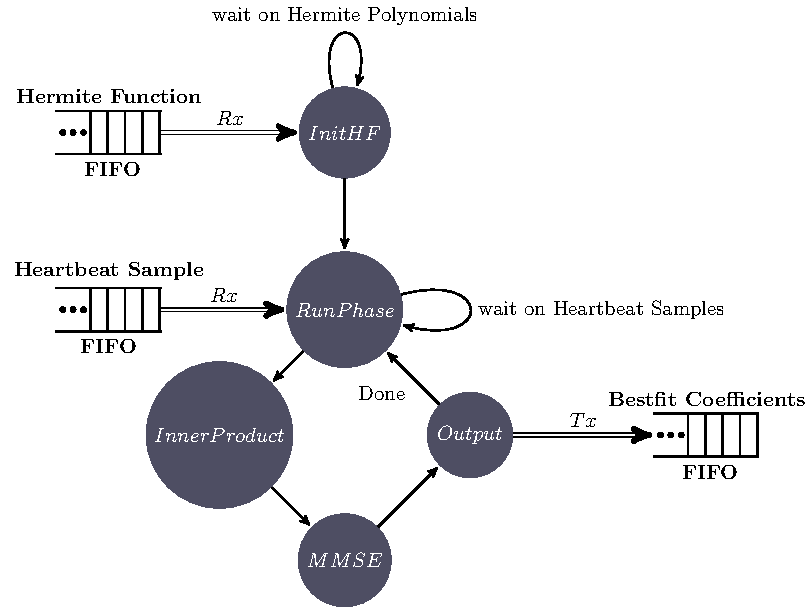
\includegraphics[scale=0.80]{stateMachine.pdf}
	\caption{Hardware Algorithm}
	\label{fig:HWAlgorithm}
\end{center}
\end{figure}

The VHDL hardware for this design is generated using AHIR-V2 toolchain \cite{c:ahir_usenix2012}.  
The generated VHDL is instantiated in the FPGA together with the RIFFA wrappers,
and the resulting design is synthesized and mapped to the Virtex-6 FPGA using
the Xilinx ISE 14.3 toolset.


%<<<<<<< HEAD
%
%HDL for this design is generated using AHIR HLS toolchain. It is equipped with a library 
%of heavily pipelined Floating Point operators and Loop Pipelining mechanism which 
%enables the final VHDL to extract parallelism in C program. It uses pipes to communicate 
%between testbench and the program, which translate to FIFOs in hardware. A simple integration 
%interface between these FIFOs and RIFFA channels completes the system. 
%
%
%The RIFFA software drivers and interface infrastructure is used to communicate between 
%host and FPGA card \cite{c:jacobsen13}. It supports upto 12 independent
%channels for data transmission. All of them end in separate Rx/Tx FIFOs on FPGA that 
%can operate on different clock domains at either ends. A simple integration 
%interface bridges RIFFA and AHIR generated FIFOs.
%By incorporating functions provided by RIFFA driver, same testbench used for 
%Software verification can be used for verifying the hardware.
%  Describe the 
%    - overall system.
%    - card
%    - the driver
%    - the hardware generation process.
%
\section{Results}\label{s:results}

We calculate round-trip delay and FPGA core power consumption for processing one beat. 
The round-trip delay is the time interval between the beginning of transmission of 
beat-data from the host to the hardware and the beginning of reception of best fit
coefficients from the hardware. 

For targeting real-time performance, size of block should be small. Also, since there 
is only 1 core operating on FPGA, having multiple beats per block will reduce only the 
communication time, which is not significant (~0.05ms average). Hence, the test feeds 
only single beat at a time to the FPGA.

In the implementation, the two loops were unrolled to different
extents to see the impact of unrolling on the system performance. 
Three levels were tried: one-way, two-way and four-way
unrolling.  The four-way unrolling gave the best performance,
as expected.  The results are summarized in Table \ref{table:Results} (the reported latency
is the average value observed across 100 beats).
%%%%%%%% Results Table %%%%%%%%%%%%%
\begin{table}[ht]
\caption{Results:  FPGA utilization and latency for different loop-unrolling levels} %title
\centering
\begin{tabular}{c @{\hskip 0.06in}| @{\hskip 0.06in}c@{\hskip 0.2in}c @{\hskip 0.2in} c @{\hskip 0.2in} c} %5 centered columns
\hline\hline\\[-1.5ex]

Unroll-level & \begin{tabular}[c]{@{}c@{}}Slice LUT  \\ Utilization  \end{tabular}& \begin{tabular}[c]{@{}c@{}}Slice Register  \\Utilization  \end{tabular}& \begin{tabular}[c]{@{}c@{}}Avg. Processing  \\Latency \end{tabular} & \begin{tabular}[c]{@{}c@{}}FPGA core Power \\ Consumption \end{tabular}\\ [2ex] \hline \\[-1.5ex]%heading

1-way & 56839 & 65995 & 1.39ms & 2.75W \\

2-way & 65895 & 80709 & 0.80ms & 2.88W \\

4-way & 84331 & 110165 & 0.44ms & 3.09W \\ [1ex]

\hline
\end{tabular}
\label{table:Results}
\end{table}
%%%%%%%%%%%%%%%%%%%%%%%%%%%

\begin{verbatim}
Minimum latency achieved with Four-way-unrolling = 0.39 ms
\end{verbatim}
It is clear that FPGA can be used for real-time processing since the 
computation time required to process single beat is much lesser than
average beat period (~1ms). The observed power dissipation is 3.1W.  
Hardware utilization in 4-way unrolled system is less than $55\%$ 
of the FPGA resource.

\subsection{Comparison with GPU/CPU implementations}

Hermite basis fitting has been evaluated on GPU and CPU implementations
as well.  For example, in \cite{c:GPU}, the authors observe that
the GPU implementation shows excellent scaling behaviour, so that 
100K beats can be processed in 15.7 seconds.  However, when it comes
to the latency needed to process a single beat, the FPGA outperforms both 
the CPU and GPU by a considerable margin, with a 35X improvement relative to
the CPU and an 11X improvement relative to the GPU. 
These comparisons are made against same algorithm executed on Intel-i7 PC(1.6GHz) 
and NVIDIA TESLA C2050 (1.15GHz). Computation frequency on Virtex-6 was kept at 100MHz which is
less than one-tenth of that on CPUs and GPUs. 

Further, the average power consumption on the FPGA is 3W as compared to $100W+$ on Core i7 processors and
$200W+$ on a GPU.  %% which GPU?
Thus, the FPGA is an attractive option for low latency ECG classification
applications in portable health monitoring devices.

\section{Conclusions}\label{s:conclusions}

In this paper, a solution to the problem of Heart Beat characterization using FPGAs is presented.
The mechanism for Hardware Generation via AHIR HLS tool and communicating with this Hardware have
been explained in detail. The automated algorithm to Hardware compilation takes away complexity
and reduces time taken for hardware design to a great extent.

This methodology is presented as an alternative to existing software oriented approaches, 
for real-time latency-sensitive signal processing. When using the FPGA, a substantial
latency reduction in single-beat processing was observed (in comparison with both
GPU and CPU implementations of the same algorithm).  
Further, the power dissipation in
the FPGA is almost two orders of magnitude lower in the FPGA implementation.

The highly parallel GPU and CPU architectures are very effective in off-line processing
(processing of a large number of beats, but not in real-time).  When it comes to real-time,
online beat processing, our work demonstrates that the FPGA offers a very competitive 
platform for ECG signal processing.

%%%% Couple of lines on Future work %%%%
 
% Bibliography
\bibliographystyle{splncs}
\bibliography{refsQRS}

\end{document}
